% vim:tw=72 sw=2 ft=tex
%         File: MF2043Summary.tex
% Date Created: 2015 Dec 17
%  Last Change: 2015 Dec 17
%     Compiler: pdflatex
%       Author: Lamn
\documentclass[12pt,a4paper]{article}
\usepackage{amsmath, amssymb}
\usepackage[utf8]{inputenc}
\usepackage[T1]{fontenc}
\usepackage[english]{babel}
\usepackage{graphicx}
\usepackage{circuitikz}
\usepackage{gb4e}

\graphicspath{{pics/}}

\title{Summary MF2043 - Robust Mechatronics}
\author{Adam Lang}

\begin{document}

\maketitle
\section{Development models}
  \subsection{V-Model}

The V-Model is used when developing new products. It is a way to model
both hardware and software and is used broadly in the industry.
It has ist name from its v-shape where the horisontal axis represents
time and the vertical axis represents level of abstraction. 

\begin{figure}[!h]
  \centering
  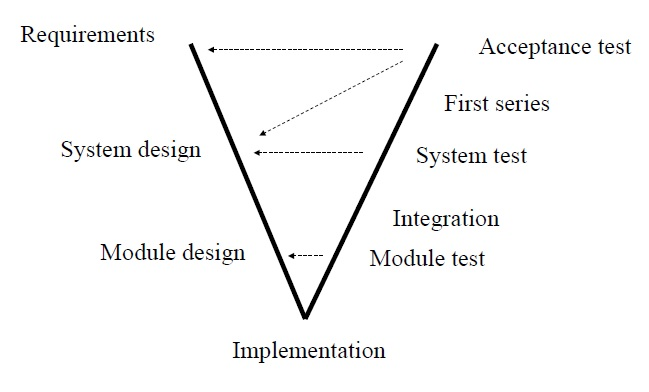
\includegraphics[scale=0.5]{VModel} 
  \caption{Graphical representation of the V-Model}
  \label{fig:Vmodel}
\end{figure}

There are seven different core activities, \textbf{Requrements analasys} 
is the first step and there are collected by analyzing the needs of the 
user(s). It is important to make the requirements measurable so that it
will be fairly easy to see if they have been fulfilled or not. The 
\textbf{system design} is where the engineers analyse the 
buisness of the proposed system from the requirements. 
Their job is to figure out the possibilities and techniques by which the requirements can be
implemented. This is more high level than the next step, \textbf{module
design} this is the lower level design where the system is broken into
smaller units or modules. Each one of them is explained in detail so the
programmer can start coding directly. At the bottom of the V we have the
\textbf{implementation} part where all the parts are implemented and put together
into one system. After the implementation step the testing starts. First
is the \textbf{module tesing} where the individual module is tested.
These are often UTPs (Unit Test Plans) and these are executed to
eliminate bugs at code level. Next is the \textbf{integration testing}
where the coexistance and communicaton of the modules is tested. The
\textbf{system testing} is done to ensure that the expectations of the
customer is met. Once the system testing is complete, ther will be a
\textbf{first series} done. After all this the final test is the
\textbf{user acceptance testing} or UAT. These tests is done in the user
enviroment it is supposed to opperate in.

\subsection{General mechatronic development}

It is important to have the whole system in mind and to look at all
diciplines when developing the system. It is important to have the
software developers develop testing frameworks for the hardware early in
the process and the mechanical designers to have the cabling in mind
when designing the mechanical system. It is also important to see the
specifications as dynamic, they will change during the work process. 

\section{Filters}
  A filter is a circut or a software that performes signal processing
  functions to remove frequency components from the signal, to enhance
  wanted ones, or both. There are many types of filters some will be
  covered below.
  \subsection{Analog}
  The analoge filter is a filter that will process the analog signal,
  comming straight from the harware. The source will often be a sensor
  of some sort, vibration, sound, temperature, extension etc. 
  \subsubsection{Anti-alias lowpass filter}
  Aliasing is an effect where different signals will become
  indestinguishable when sampled. If a signal with noise is sampled
  there will be no way of differentiatiating the noise from the signal.
  There is a variety of implementations for when a analog signal will 
  be digitilized, audio beeing one of the most intuitive. The convertion
  between analog and digital is done by sampling the amplitude of the
  analog signal and convert each sample to a numeric quantity. This
  process can introduce artefacts, or missleading amplitudes due to both the
  finite accuracy by which the values are quantizied and brought from
  the continuos to the descrete and from the finite rate at which these
  samples are taken. The \textbf{Nyqvist criterion} says that the signal
  beeing digitilized can not contain frequencies that exceeds half the
  sampling rate $f_s$. This is usualy accomplished by passing the signal
  through a \textbf{anti-aliasing filter} whose cutoff frequency $f_c$
  ensures thorough attenuation of signals above the Nyqvist frequency
  $f_s/2$. In short the banwidth of the signal is restricted to satisfy
  the samplin theorem that states that the unambiguous reconstruction of
  the signal from its samples is possible if the power of the
  frequencies over the Nyqvist criterion is zero. In real life it is a
  trade off between bandwidth and aliasing. 
  \begin{exe}
    \ex Example: \\
    You have a signal from a sensor that you are sampling at $f_s = 1kHz$.
    What should be you cutoff frecuency $f_c$? \\
    \textbf{Answer:} $f_c = f_s/2 = 500 Hz$ Due to the Nyqvist criterion.
  \end{exe}
  \subsubsection{Passive filters}
  There are a veriety of different passive filters both high- and low
  pass. The simpelest filters are presented below.
  \begin{figure}[!h]
  \begin{center}
      \begin{circuitikz}[european]
        \draw(0,0)
        to[short, o-] (2,0) 
        to[C=$C$, *-*] (2,2)
        to[R=$R$, -o] (0,2)
        to[open, v>=$V$,o-o] (0,0);
        
        \draw(2,0)
        to[short] (4,0)
        to[open, v=$V$, o-o] (4,2)
        to[short] (2,2);

      \end{circuitikz}
      \caption{Low Pass RC filter}
    \end{center}
  \end{figure}
            



    



    \subsubsection{Active Filters}


\end{document}
